\documentclass{ctexart}

\usepackage{graphicx}
\usepackage{float}
\usepackage{amsmath}
\usepackage{listings}
\usepackage{xcolor}

\lstset{
    language=Verilog,          % 设置语言为 Verilog
    basicstyle=\ttfamily\small,% 字体与字号
    keywordstyle=\color{blue}\bfseries, % 关键字（如 module, input, output）加粗变蓝
    commentstyle=\color{gray}\itshape,  % 注释（// 或 /* */）斜体变灰
    stringstyle=\color{red},     % 字符串颜色
    numbers=left,              % 行号显示在左侧
    numberstyle=\tiny\color{gray}, % 行号的字体和颜色
    stepnumber=1,              % 行号每行都显示
    numbersep=8pt,             % 行号与代码的距离
    backgroundcolor=\color{white}, % 代码块背景色
    showspaces=false,          % 不显示空格
    showstringspaces=false,    % 不显示字符串中的空格
    showtabs=false,            % 不显示 Tab 符号
    frame=single,              % 给代码块加一个单线边框
    rulecolor=\color{black!30},% 边框颜色（浅黑）
    tabsize=4,                 % Tab 键相当于 4 个空格
    captionpos=b,              % 代码标题位置（b=底部，t=顶部）
    breaklines=true,           % 开启自动折行（防止代码太长超出页面）
}


\title{Computer Organization LAB}
\date{\today}
\author{计算机2405 邵凯伟}

\begin{document}

\maketitle
\tableofcontents

\newpage

\setcounter{section}{-1}

\section{环境搭建}
\subsection{logisim}
\noindent
直接下载
\subsection{verilog}
\noindent
采用iverilog + surfer方案

\includegraphics[width = 0.05\textwidth]{surfer.png}\\
使用\verb|iverilog -o output code1.v code2.v|编译\\
使用\verb|vvp output|模拟运行，（Verilog Virtual Processor）\\
使用\verb|surfer filename.vcd|查看波形\\
surfer原料:在仿真文件中加入
\begin{verbatim}
initial begin
    $dumpfile("filenae.vcd");
    $dumpfile(0, modulename);
end
\end{verbatim}
生成vcd文件\\
输出示例：
\begin{figure}[H]
    \centering
    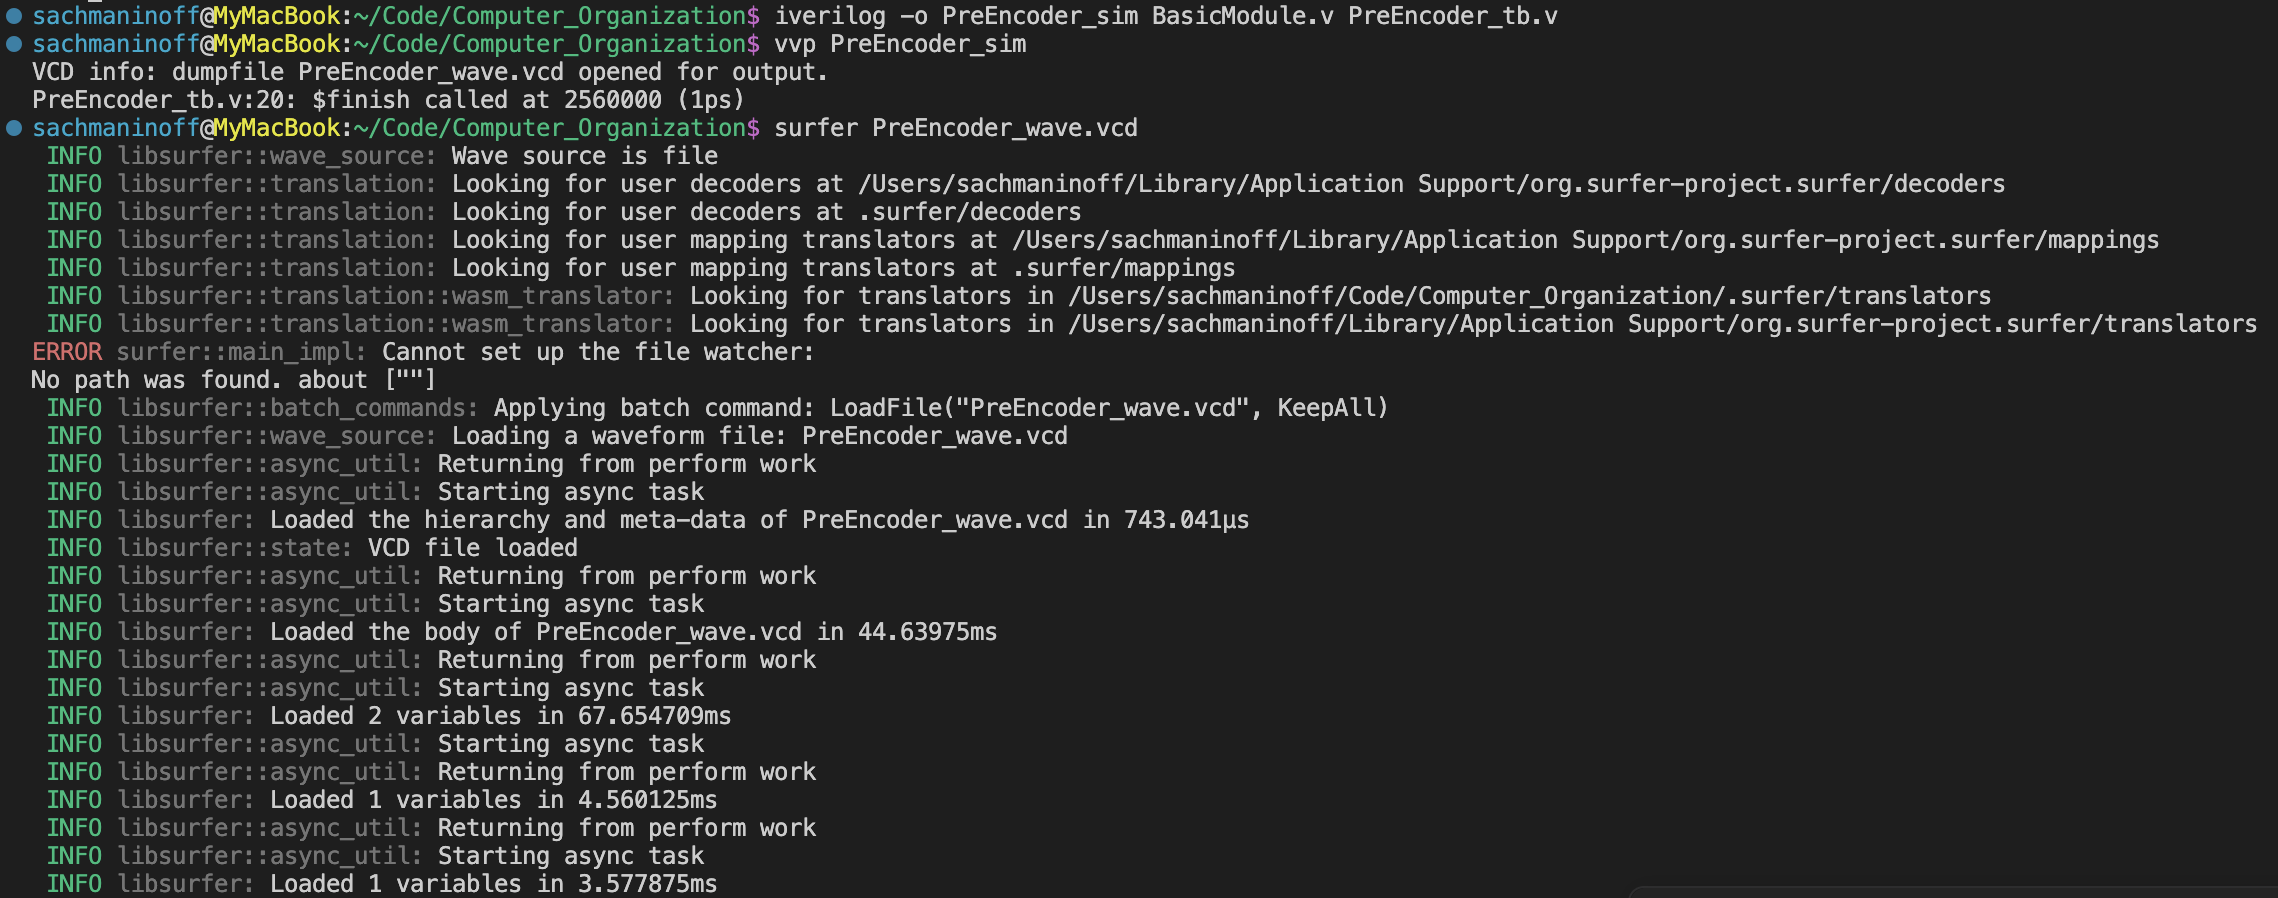
\includegraphics[width = 0.75\textwidth]{example_output.png}
\end{figure}
\section{实验一\ 组合电路设计}
\noindent
基础门电路设计：多输入门电路, 复用器\\
基础功能模块设计：编码器, 译码器、、

\subsection{logisim实现}
\subsubsection{多路复用器}
\textbf{二路复用器}\\
如图\ref{MUX_2}。
\begin{figure}[h]
    \centering
    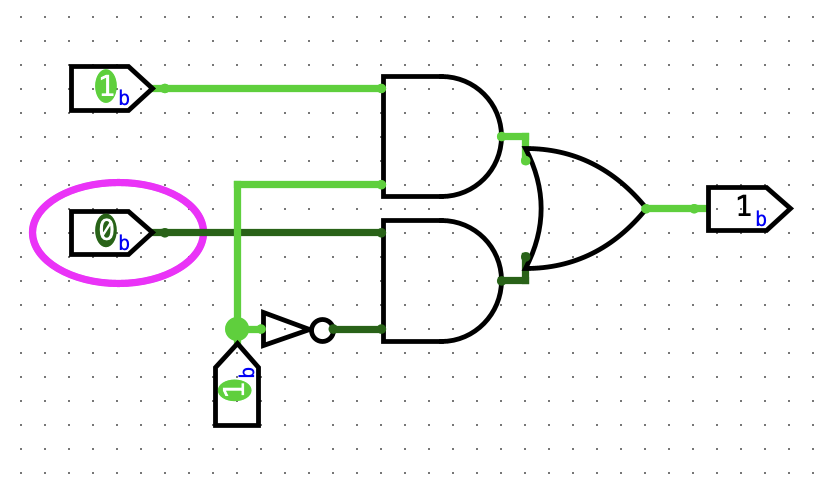
\includegraphics[width = 0.45\textwidth]{MUX_2.png}
    \caption{二路复用器}
    \label{MUX_2}
\end{figure}

\textbf{三态门实现二路复用器}\\
如图\ref{MUX_2_3}，用三态门代替与门，复用三态门线与省略或门。
\begin{figure}[h]
    \centering
    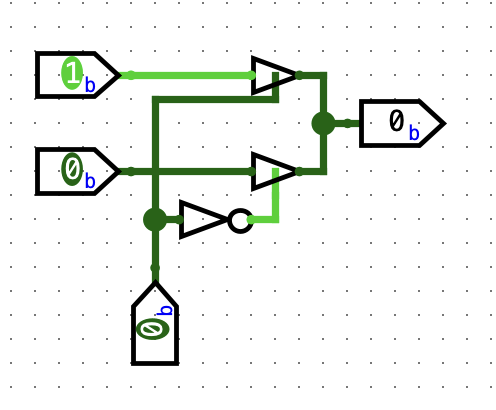
\includegraphics[width = 0.45\textwidth]{MUX_2_3.png}
    \caption{三态门二路复用器}
    \label{MUX_2_3}
\end{figure}

\textbf{四路复用器}\\
采用两层二路复用器实现，如图\ref{MUX_4}。
\begin{figure}[h]
    \centering
    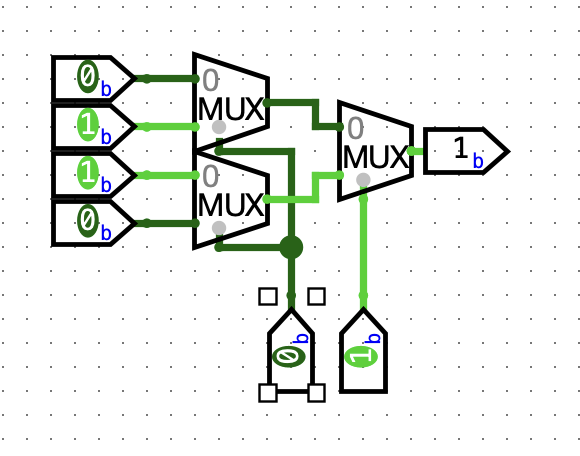
\includegraphics[width = 0.45\textwidth]{MUX_4.png}
    \caption{四路复用器}
    \label{MUX_4}
\end{figure}

\subsubsection{编码器}
\textbf{8-3编码器}\\
根据真值表，只需进行或逻辑：\\
$$
\begin{cases}
    Y_2=I_4+I_5+I_6+I_7\\
    Y_1=I_2+I_3+I_6+I_7\\
    Y_0=I_1+I_3+I_5+I_7
\end{cases}
$$
实现如图\ref{Encoder_83}。
\begin{figure}[h]
    \centering
    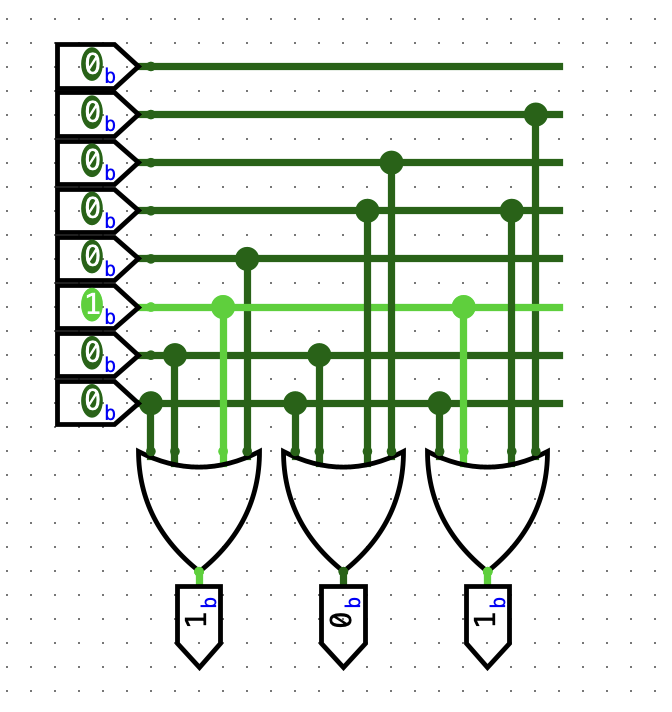
\includegraphics[width = 0.45\textwidth]{Encoder_83.png}
    \caption{8-3编码器}
    \label{Encoder_83}
\end{figure}

\textbf{8-3优先编码器}\\
逻辑分为两部分：仅点亮最高优先级的数据线，普通8-3编码器。\\
优先级部分：每一个输入$D_k$取决于$D_0$~$D_{k-1}$的非的与，再与上$I_k$（图\ref{PreEncoder_83}中的七个与门），非之与部分可变为或非门，
（图中两个或非门用于简化低位逻辑），避免使用过多输入的与门。最后三个或门为普通8-3编码器。
\begin{figure}[h]
    \centering
    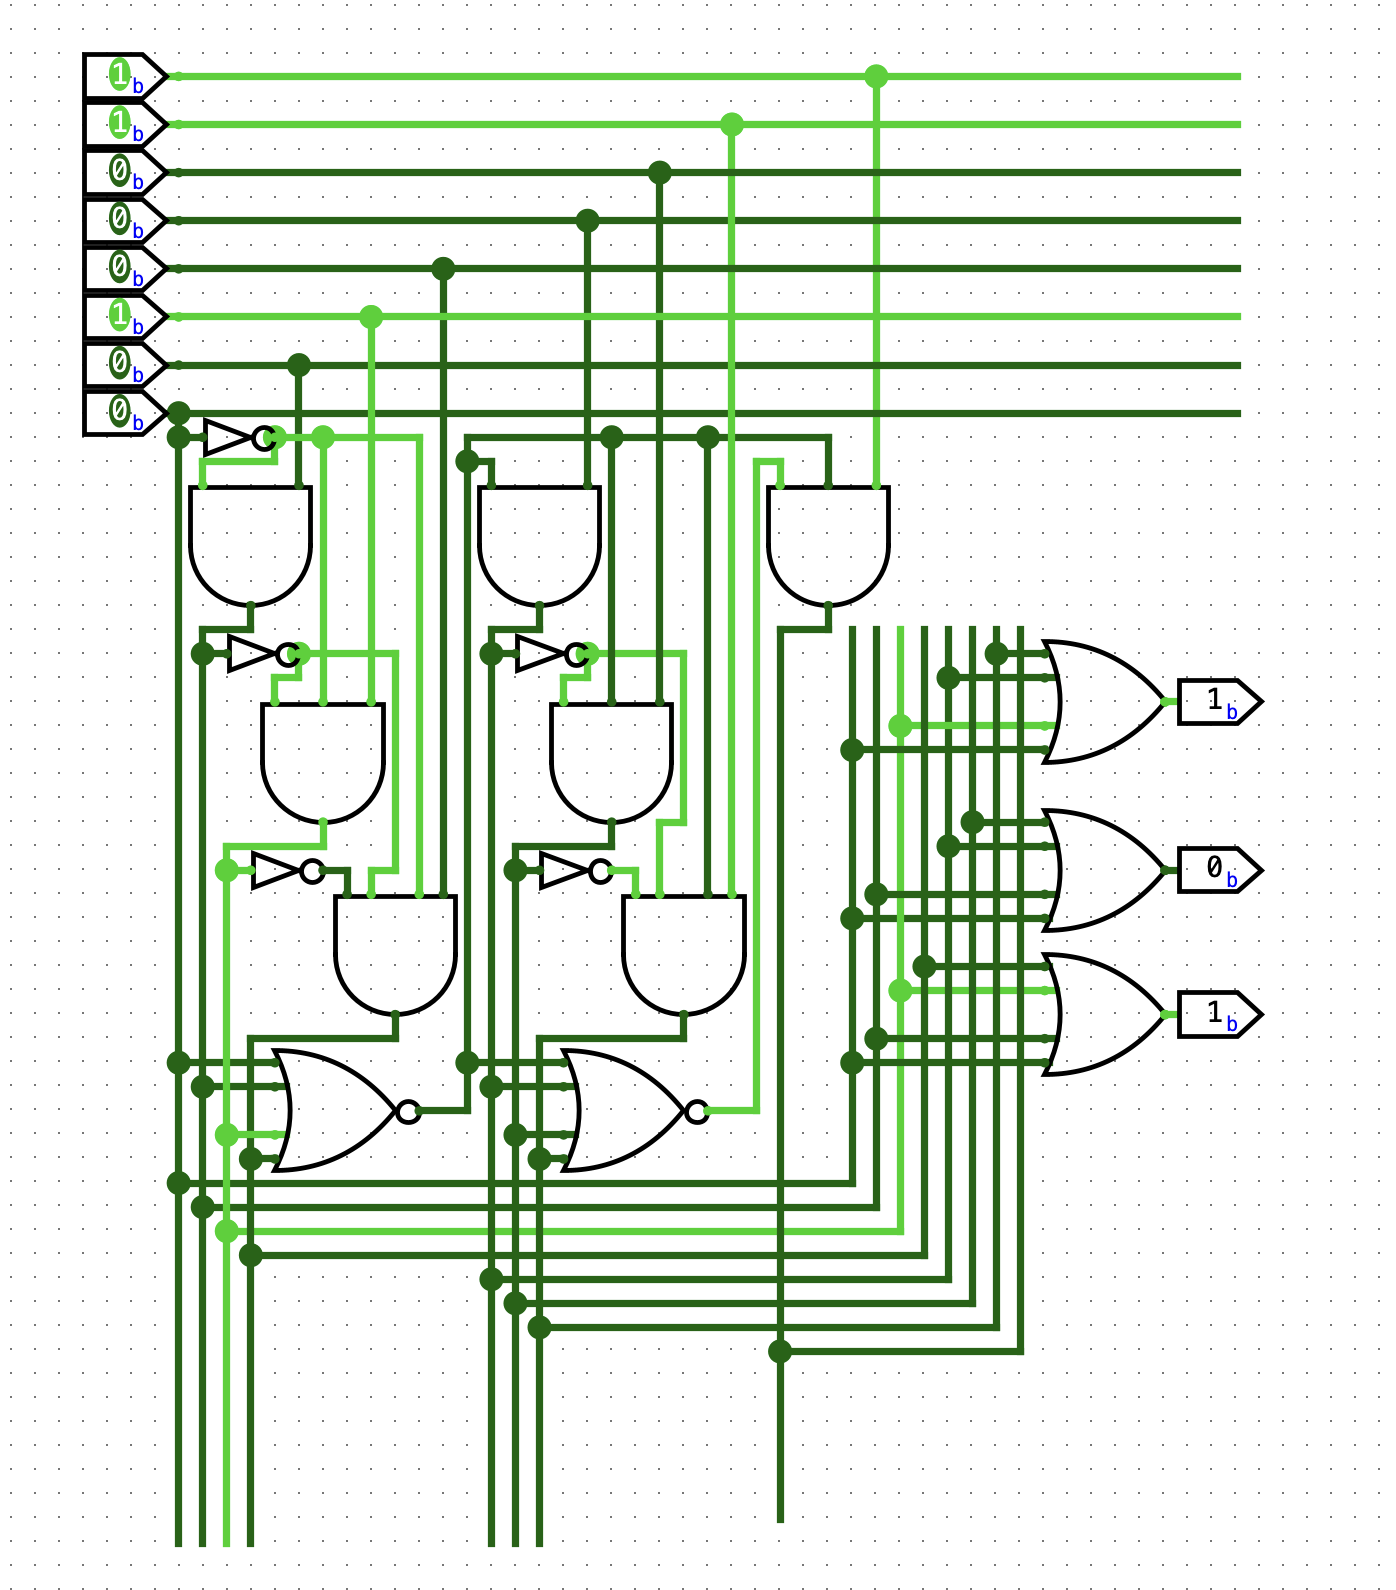
\includegraphics[width = 0.7\textwidth]{PreEncoder_83.png}
    \caption{8-3优先编码器}
    \label{PreEncoder_83}
\end{figure}

\subsubsection{译码器}
\textbf{3-8译码器}\\
如图\ref{Decoder_38}, 使用与阵列即可。
\begin{figure}[h]
    \centering
    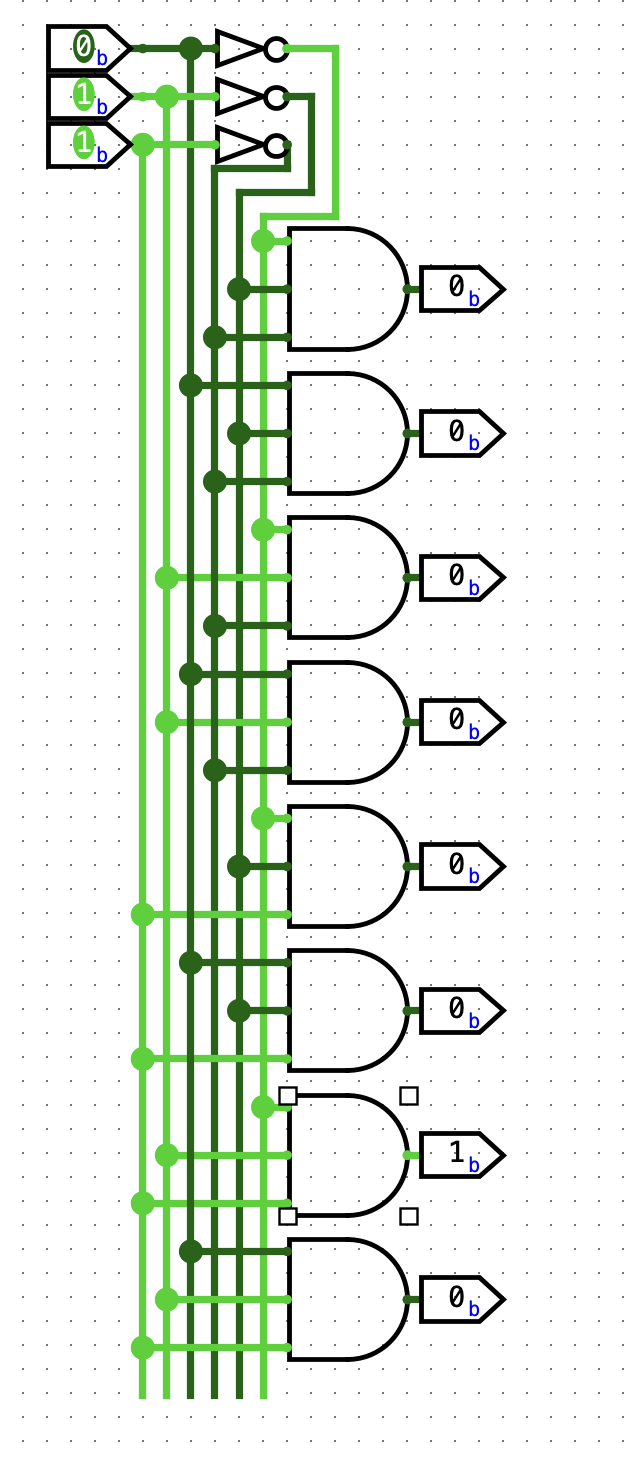
\includegraphics[width = 0.45\textwidth]{Decoder_38.png}
    \caption{3-8译码器}
    \label{Decoder_38}
\end{figure}

\subsection{verilog实现}
\subsubsection{多路复用器}
\noindent
使用参数化路数量\verb|#(parameter ways = 4)|，易于复用代码\\
\verb|$clog2()|为内置函数，选择位宽为输入位宽的对数\\
最后将\verb|data_in[sel]|作为输出即可。
\begin{lstlisting}[caption = {多路复用器}]
module MUX #(
    parameter ways = 4
) (
    input wire [ways - 1 : 0] data_in,
    input wire [$clog2(ways) - 1 : 0] sel,
    output wire data_out
);
    assign data_out = data_in[sel];
endmodule
\end{lstlisting}
\subsubsection{优先编码器}
\noindent
输出在\verb|always|块中赋值，将\verb|wire|改为\verb|reg|，用\verb|flag|模拟\verb|break|语句。\\
在\verb|for|循环外先给\verb|data_out|赋初值，以防止\verb|data_in|全为0时\verb|data_out|变为寄存器.
\begin{lstlisting}[caption = {优先编码器}]
module PreEncoder #(
    parameter ways = 8
) (
    input wire [ways - 1 : 0] data_in,
    output reg [$clog2(ways) - 1 : 0] data_out
);
    reg flag;
    integer i;
    always @(*) begin
        flag = 0;
        i = 0;
        data_out = 0;
        for (i = ways - 1; i >= 0; i = i - 1)  begin
            if (!flag) begin
                if (data_in[i]) begin
                    flag = 1;
                    data_out = i;
                end
            end
        end
    end
endmodule
\end{lstlisting}
\subsubsection{译码器}
\noindent
\verb|data_out|的第\verb|data_in|位为1，其余均为0。\\
故\verb|data_out = 1 << data_in|。
\begin{lstlisting}[caption = {译码器}]
module Decoder #(
    parameter ways = 8
) (
    input wire [$clog2(ways) - 1 : 0] data_in,
    output wire [ways - 1 : 0] data_out
);
    assign data_out = 1'b1 << data_in;
endmodule
\end{lstlisting}
\subsection{verilog仿真}
\subsubsection{优先编码器}
\begin{lstlisting}[caption = {优先编码器仿真}]
`timescale 1ns / 1ps
module PreEncoder_tb;
    parameter ways = 8;
    reg [ways - 1 : 0] data_in;
    wire [$clog2(ways) - 1 : 0] data_out;

    integer i;

    PreEncoder #(
        .ways(ways)
    ) PreEncoder_sim (
        .data_in(data_in),
        .data_out(data_out)
    );
    initial begin
        for (i = 0; i < (1 << ways); i = i + 1) begin
            data_in = i;
            #10;
        end
        $finish;
    end
    initial begin
        $dumpfile("PreEncoder_wave.vcd");
        $dumpvars(0, PreEncoder_tb);
    end
endmodule
\end{lstlisting}

\textbf{波形图}
\begin{figure}[h]
    \centering
    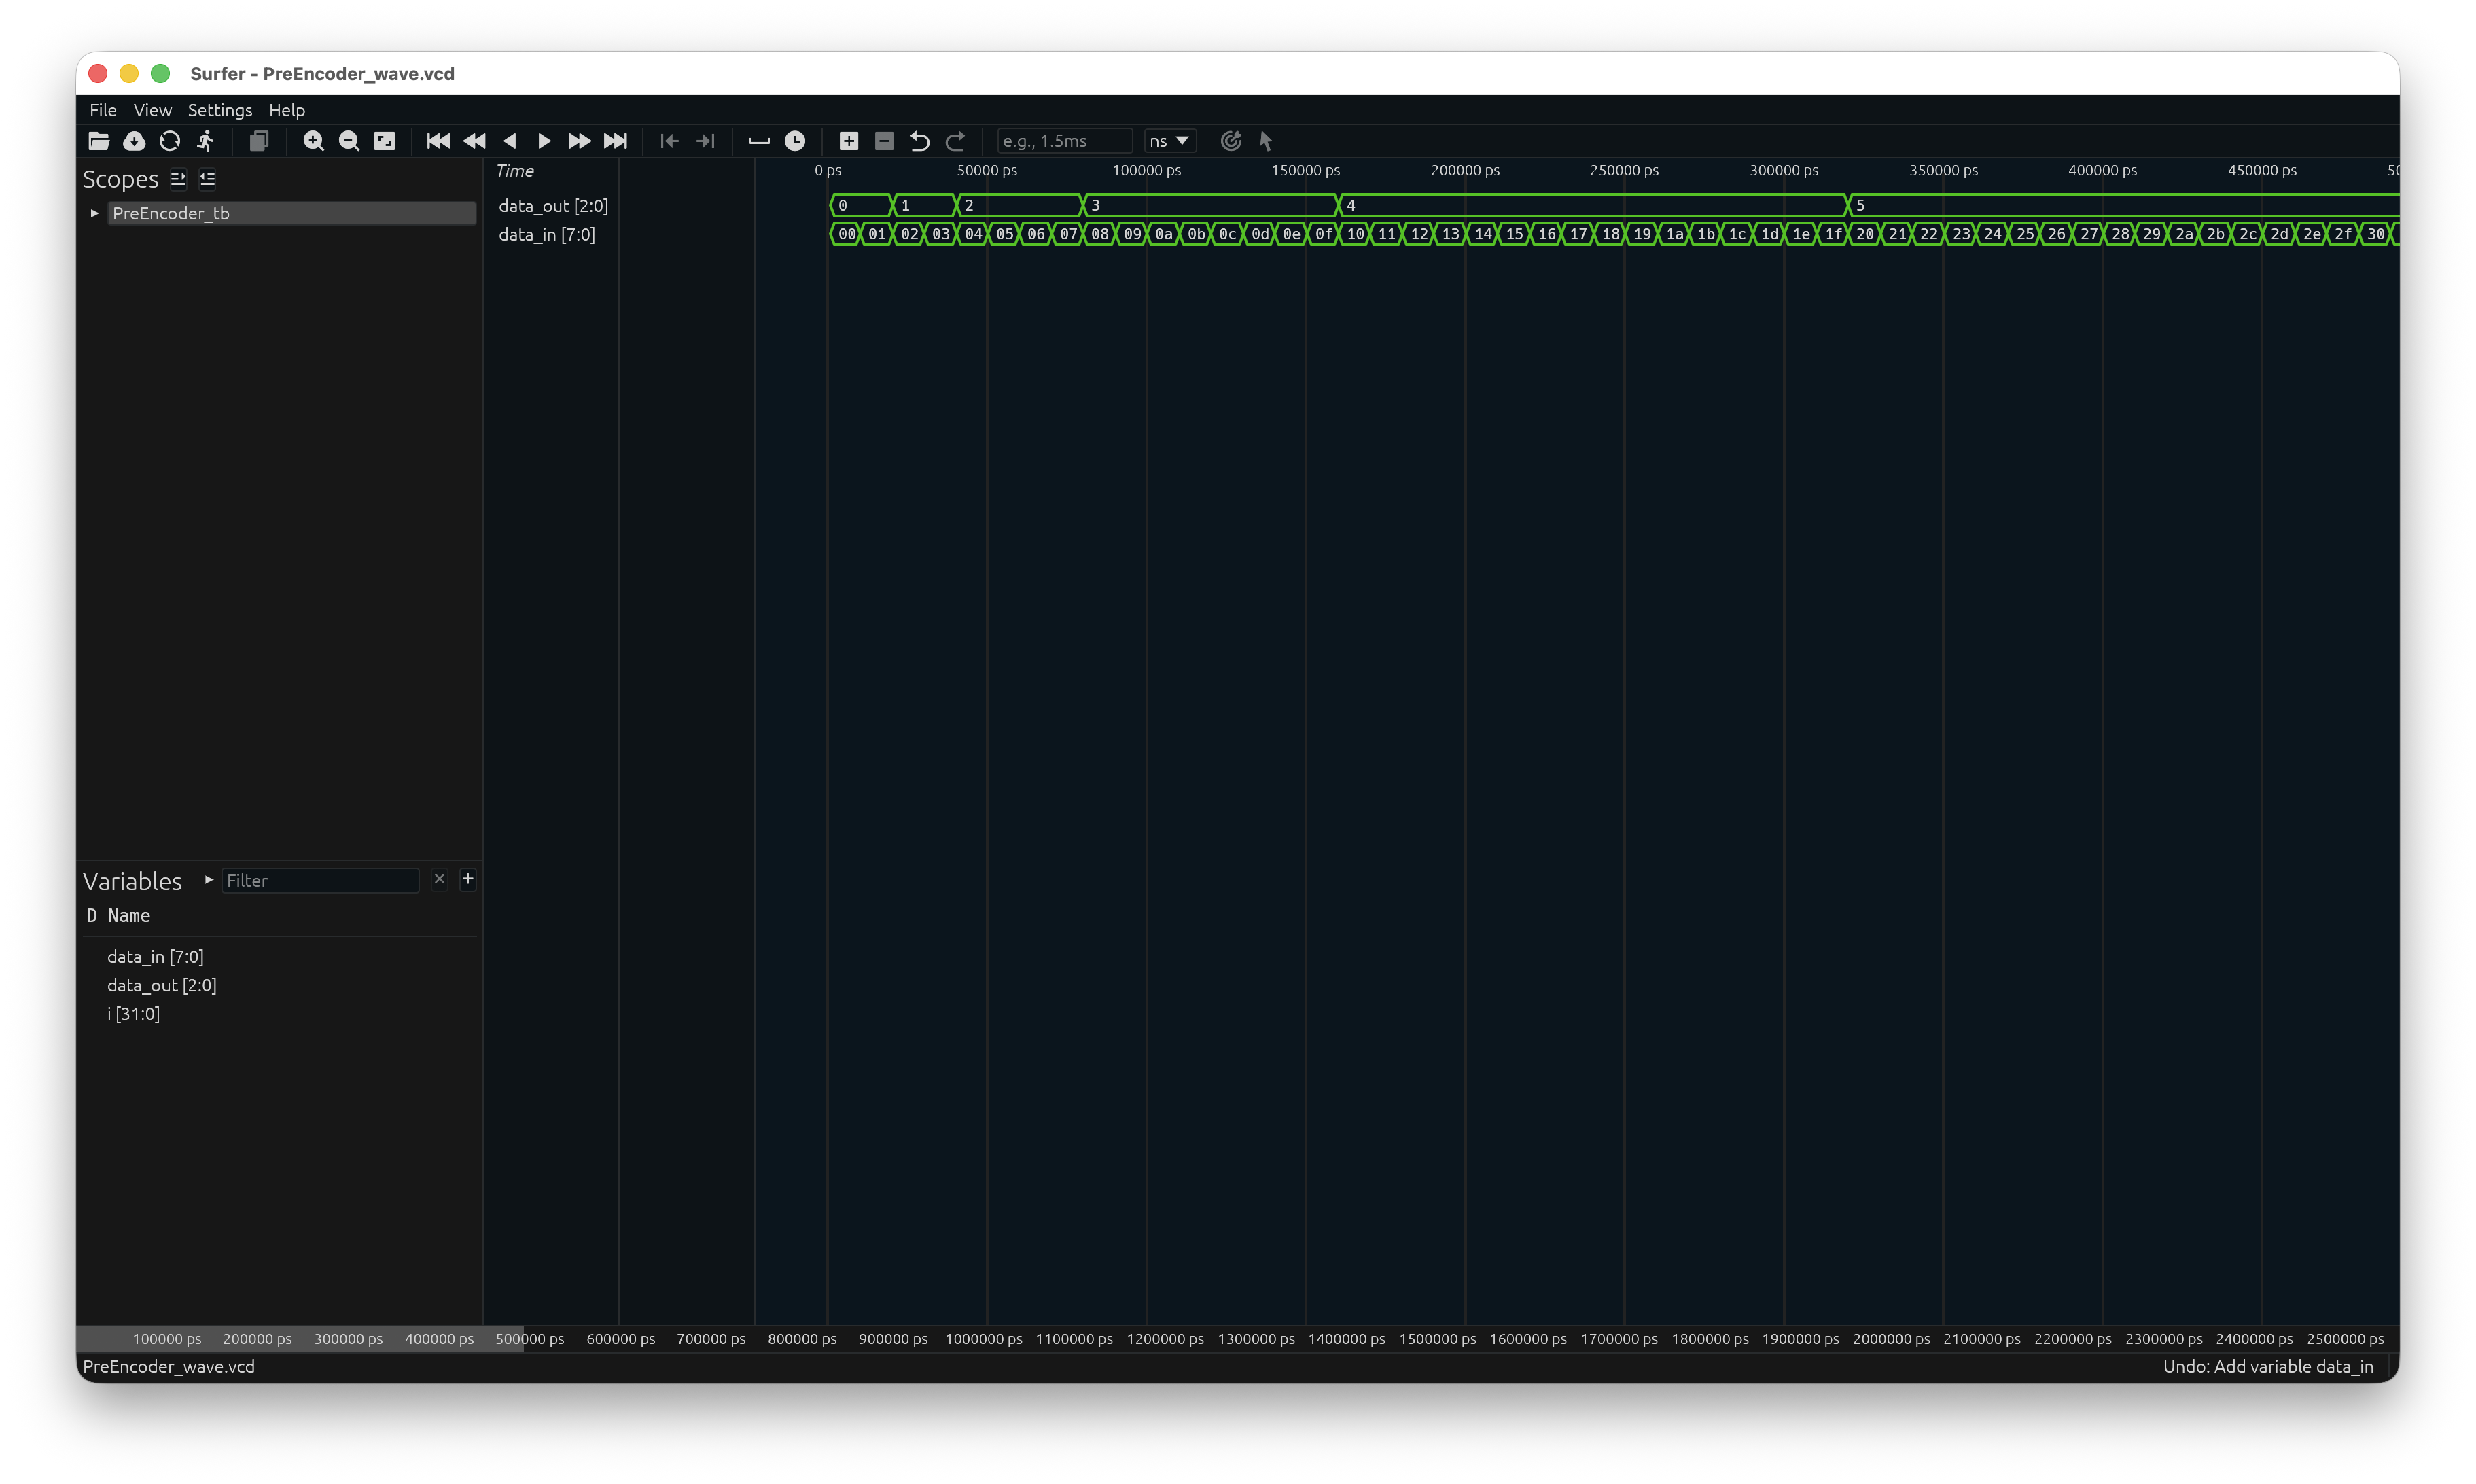
\includegraphics[width = \textwidth]{PreEncoder_wave.png}
    \caption{优先编码器仿真波形}
\end{figure}
\subsubsection{译码器}
\begin{lstlisting}[caption = {编码器仿真}]
`timescale 1ns / 1ps
module Decoder_tb;
    parameter ways = 8;
    reg [$clog2(ways) - 1 : 0] data_in;
    wire [ways - 1 : 0] data_out;

    integer i;

    Decoder #(
        .ways(ways)
    ) Decoder_sim (
        .data_in(data_in),
        .data_out(data_out)
    );
    initial begin
        for (i = 0; i < ways; i = i + 1) begin
            data_in = i;
            #10;
        end
        $finish;
    end
    initial begin
        $dumpfile("Decoder_wave.vcd");
        $dumpvars(0, Decoder_tb);
    end
endmodule
\end{lstlisting}

\textbf{波形图}
\begin{figure}[h]
    \centering
    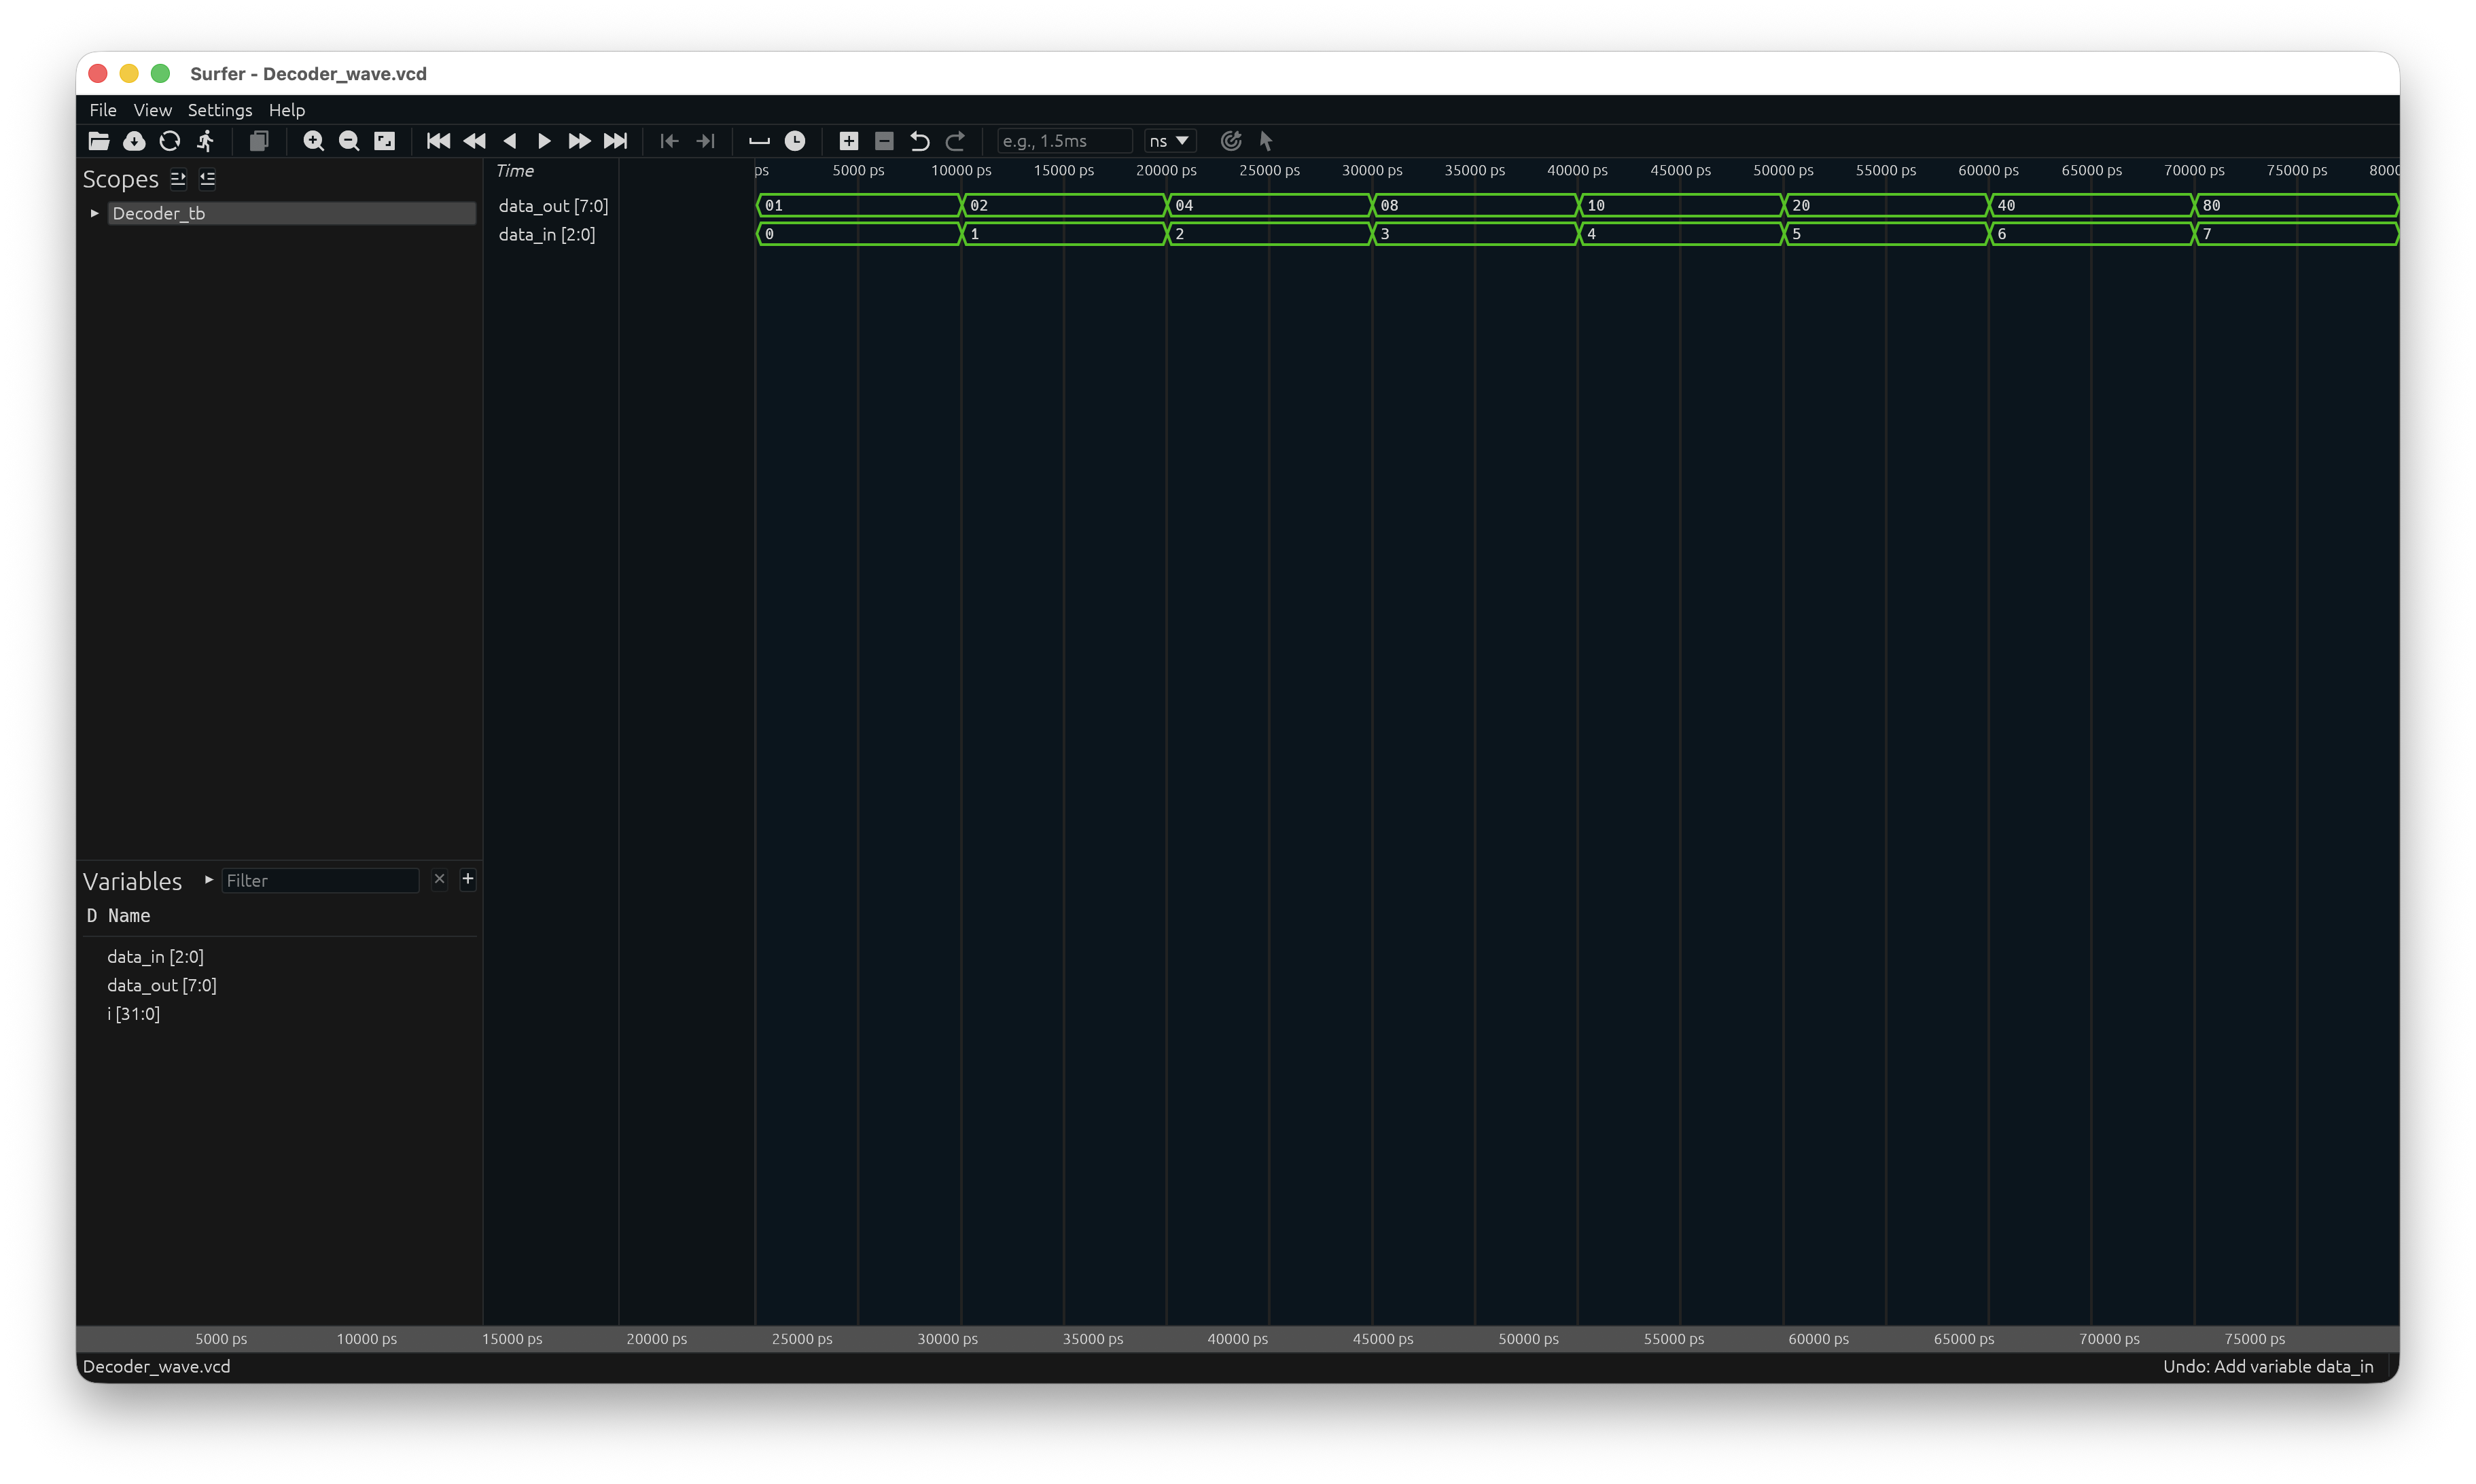
\includegraphics[width = \textwidth]{Decoder_wave.png}
    \caption{译码器仿真波形}
\end{figure}

\end{document}